
%% CLASS MANUAL FOUND IN http://blog.poormansmath.net/latex-class-for-lecture-notes/ %%
%% CLASS AUTHOR Stefano Maggiolo %%
\documentclass[english,course]{Notes}

\title{ INTRODUCTORY ECONOMICS}
\subject{Economics}
\author{Joao Almeida-Domingues}
\email{2334590D@student.gla.ac.uk}
\speaker{Dr. Constantine Sorokin}
\date{07}{01}{2019}
\dateend{24}{05}{2019}
\place{University of Glasgow}
\usepackage[backend=biber, style=reading]{biblatex}
\bibliography{refEco}
\usepackage{csquotes}
\newcommand\quo[1]{\begin{displayquote}\ita{\large{#1}}\end{displayquote}}



 %%%%% GENERAL MATHEMATICAL NOTATION SHORTCUTS %%%%%
 
\newcommand{\n}{\mathbb{N}}
\newcommand{\z}{\mathbb{Z}}
\newcommand{\q}{\mathbb{Q}}
\newcommand{\cx}{\mathbb{C}}
\newcommand{\real}{\mathbb{R}}
\newcommand{\field}{\mathbb{F}}
\newcommand{\ita}[1]{\textit{#1}}
\newcommand{\oneton}{\{1,2,3,...,n\}}
\newcommand\ef{\ita{f} } 
\newcommand\inv[1]{#1^{-1}}
\newcommand\setb[1]{\{#1\}}
\newcommand\en{\ita{n }}
\renewcommand\qedsymbol{QED} %\qedhere to force QED in place

%%%%%%%%%%%%%%%%PACKAGES%%%%%%%%%%%%%%%%%%%%%%%%%%%%%
\usepackage{lipsum}  
\usepackage{amsmath,amsthm,amssymb,graphicx,mathtools,tikz,pgfplots} %maths
\usepackage{hyperref,framed,color,fancybox} %layout
% framed :  \begin{shaded,frame,snugshade or leftbar} \definecolor{shadecolor}{rgb}{XYZ} to change color
%fancybox: \shadowbox,ovalbox or doublebox
%%%%%%%%%%%%%%%%%%%%%%%%%%%

%%%CLASS SHORTCUTS%%%%
%\lecture{day}{month}{year} for margin note
%\begin{theorem} sdfsdf\end{theorem}
%\begin{proposition} dfsdfs\end{proposition}
%\begin{lemma} dsfsd \end{lemma}
%\begin{corollary} f ffew \end{corollary}
%\begin{definition} fwewef w \end{definition}
%\begin{example} feww e\end{example}
%\begin{exercise} wefwe \end{exercise}
%\begin{remark} wef we \end{remark}
%\begin{fact} wefe \end{fact}
%\begin{problem} wef ew \end{problem}
%\begin{conjecture} ewfew \end{conjecture}
%\begin{claim} few w \end{claim}
%\begin{notation} fewf \end{notation}

\begin{document}
\newpage

\section{Microeconomics}

\subsection{Introduction}

\lecture{08}{01}{2019}
We start our journey into the science of economics by establishing its first principles. In particular, we'll focus on:

\begin{itemize}
	\item How individuals make choices?
	\item How individual choices interact?
	\item How those interactions, when combined, give rise to much more complex \ita{economy-wide} interactions
\end{itemize}

\defn{Economy}{A system for coordinating society's productive activities}

\defn{Economics}{The science which studies the production, distribution and consumption of goods}

\par{Most modern day economies are \ita{market economies} \ref{intro:market}, instead of being centrally controlled by an institution \ref{intro:command}, their organisation rely on the many firms and individuals' decisions (in general, people produce and buy whatever they feel like). Adam Smith first observed how this system of individuals making isolated decisions in pursuit of their own interests \ref{intro:hand} could bring about gains to society as a whole in his 1776 \ita{magnum opus - The Wealth of Nation}. In this work he coined the now ubiquitous term of the \ita{invisible hand}.}

\quo{... every individual necessarily labours to render the annual revenue of the society as great as he can. He generally, indeed, neither intends to promote the public interest, nor knows how much he is promoting it. By preferring the support of domestic to that of foreign industry, he intends only his own security; and by directing that industry in such a manner as its produce may be of the greatest value, he intends only his own gain, and he is in this, as in many other cases, led by an invisible hand to promote an end which was no part of his intention.}

\defn{Market Economy}{Decisions about production and consumption are made by individual producers and consumers~\label{intro:market}}

\defn{Command Economy}{The government determines what goods should be produced, how much should be produced and the price at which the goods are offered for sale~\label{intro:command}}

\defn{Invisible Hand}{The way in which the individual pursuit of self-interest can lead to good results for society as a whole~\label{intro:hand}}

\defn{Microeconomics}{The branch of economics that studies how people make decisions and how these interact}



\par{Things don't always go smoothly when the invisible hand is the only guiding force in action. When the individuals' pursuit of self-interest brings about detrimental effects to society, economies experience \ita{market failure~\ref{intro:failure}}. An aggregate of these failures can lead to entire periods of general ill-being~\ref{intro:rec}. These fluctuations between periods of greater~\ref{intro:growth} and lesser wealth are , however,  a common feature of modern economies which macroeconomists occupy themselves with~\ref{intro:macro}}

\defn{Macroeconomics}{The branch of economics that studies the overall ups and downs in the economy as a whole~\label{intro:macro}}

\defn{Market Failure}{When the individual pursuit of self-interest leads to bad results for society as a whole~\label{intro:failure}}

\defn{Recession}{A downturn in the economy~\label{intro:rec}}

\defn{Economic Growth}{The growing ability of the economy to produce goods and services~\label{intro:growth}}

\subsection{Underlying Principles of Individual Choice}

\begin{enumerate}
	
	\item{Scarce resources mandate choices}
	\item{The true cost of an item is its opportunity cost~\ref{principles:cost}}
	\item{"How Much" decisions, require making \ita{trade-offs}~\ref{principles:trade-off} at the margin~\ref{principles:margin}}
		\rem{Not all decisions are binary, some involve assessing the costs and benefits at different stages (e.g. dropping out of college in your last semester vs first)}
	\item{People usually respond to incentives~\ref{principles:incentive}, exploiting opportunities to make themselves better off~\label{principles:incentiveP}}
		\rem{the principle that people will exploit opportunities to make themselves better off is the basis of all predictions by economists about individual behaviour}
	

	\defn{Opportunity Cost}{What you must give up in order to get something else~\label{principles:cost}}
	\defn{Trade-Off}{Comparing the costs and benefits of a choice~\label{principles:trade-off}}
	\defn{Marginal Decisions}{Decisions that occur at the cost-benefit margin~\label{principles:margin}}
	\defn{Marginal Analysis}{The study of marginal decisions}
	\defn{Incentive}{Anything which rewards behaviour changes~\label{principles:incentive}}
	
\subsection{Principles of the Interaction of Individual Choices}



	\item{Specialisation brings about gains from trade}
	\item{Markets move towards equilibrium~\ref{principles:equilibrium}}
		\rem{This follows from \ref{principles:incentiveP}}
	\item{Resources should be used efficiently to achieve society's goals}
		\rem{Occasionally there are overriding reasons to efficiency, like equity~\ref{principles:equity}}
	\item{Markets tend towards efficiency}
	\item{When markets don?t achieve efficiency, government intervention can improve society?s welfare}
	
\subsection{Principles of Economy-Wide Interactions}

	\item{One person's spending is another's income}
		\rem{In a recession, for example, this causes a synergic effect. People lose jobs, they have less money, they spend less, other people have less, they also lose their jobs etc.}
	\item{Overall Spending Sometimes Gets Out of Line with the Economy?s Productive Capacity}
		\rem{Underspending often leads to recessions. Overspending leads to \ita{inflation}~\ref{principles:inflation}}
	\item{Government Policies Can Change Spending}
	
\end{enumerate}
	
	\defn{Equilibrium}{A situation in which individuals cannot make themselves better off by doing something different~\label{principles:equilibrium}}
	\defn{Efficient Economy}{Resources are used efficiently when they are used in a way that has fully exploited all opportunities to make everyone better off~\label{principles:equilibrium}}
	\defn{Equity}{Allowing for everyone to have his/her fair share~\label{principles:equity}}
	\defn{Inflation}{A rise in prices throughout the economy. This occurs because when the amount that people want to buy outstrips the supply, producers can raise their prices and still find willing customers.~\label{principles:inflation}}
	
\section{Economic Models}
\lecture{09}{01}{2019}

In this section:
\begin{enumerate}
	\item Explain the crucial role that models play in economics
	\item Introduce 2 simple models: comparative advantage ; possibility frontier
	\item Explain the difference between normative and positive economics
\end{enumerate}

\defn{Model}{ Simplified representation of reality that is used to better understand real-life situations}
	\rem{Models are essential to economics, because their relative simplicity allow economists to hold everything else constant and study how one change affects the overall economic outcome}
	
\defn{Production Possibility Frontier Model}{A curve depicting all maximum output possibilities for two goods, given a set of inputs consisting of resources and other factors. The PPF assumes that all inputs are used efficiently}

\par{The PPF model helps companies evaluate their \ita{production efficiency}. When a company its producing at its \ita{production possibility frontier~\ref{model:ppf}} we say that it is \ita{efficient in production~\ref{model:efProd}}. This however is not enough to classify an economy as efficient. After the goods are produced it is necessary to produce the mix of goods that people want to consume, if this is the case we talk of \ita{efficient in allocation~\ref{model:efAl}}}

\defn{PPF}{The limit at which an economy as maximised the usage of resources, maximising its production capacity~\label{model:ppf}}
\defn{Efficient in Production}{When an economy is in its production possibility frontier; we say that the economy is efficient in production~\label{model:efProd}}
\defn{Efficient in Allocation}{When an economy allocate its resources so that consumers are as well off as possible~\label{model:efAl}}

\begin{figure}[h]
\centering
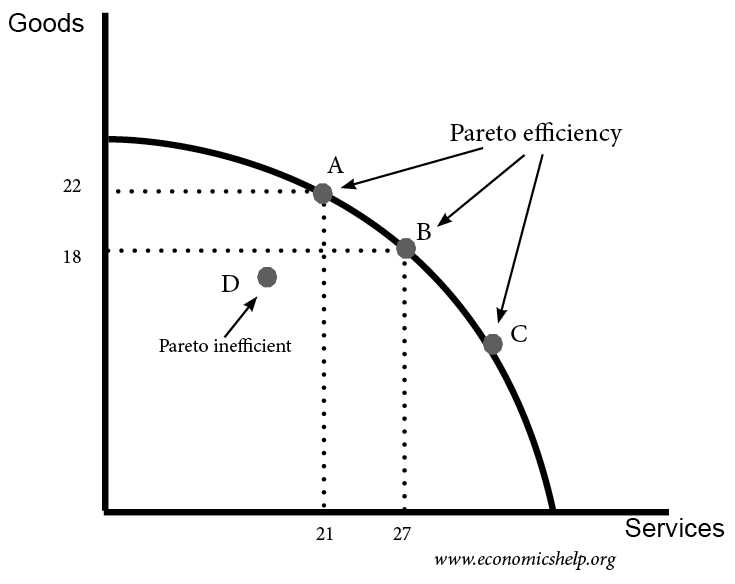
\includegraphics[width=0.8\textwidth]{assets/ppf.png}
\end{figure}

\par{We can estimate the \ita{opportunity cost} of producing different goods by looking at the gradient of the line between the current point and the point we wish to investigate. The steeper the gradient (for greater $\Big|\frac{\mathrm{d}y}{\mathrm{d}x}\Big| $), the higher the opportunity cost}

\par{We can also look at the \ita{economic growth}. Economic growth means an expansion of the economy's production possibilities. Hence we should expect the graph to be scaled in all directions. This can come about due to an increase in the \ita{factors of production~\ref{model:prod}} (e.g. new hangar, whereby a company can produce more aircrafts of type A without reducing the number of type Bs). Or by advances in \ita{technology}(e.g. semicondutors industry, transistors, home pc)}

\defn{Factors of Production}{Any resource needed for the creation of a good or service (land, labor, capital and entrepreneurship)~\label{model:prod}}



\lecture{10}{01}{2019}





\newpage
\nocite{*}
\printbibliography

\end{document}